\documentclass[11pt,svgnames,smaller]{beamer}

\usepackage{CommandsAndStyle}

\usepackage{listings}
\usepackage{amsthm}
\usepackage{amsmath}
\usepackage{subfig}
\usepackage{xcolor}
\usepackage{textpos}
\usepackage{transparent}
\usepackage{tikz}
\usepackage{epigraph}

\usepackage{array, makecell} %

\usepackage{caption}
\captionsetup[figure]{labelformat=empty}% redefines the caption setup of the figures environment in the beamer class.

\newcommand{\fsamp}{\textsc{F-samp}\xspace}
\newcommand{\base}{\textsc{base}\xspace}
\newcommand{\fcount}{\textsc{F-count}\xspace}
\mode<presentation>

\author{Gaspare Ferraro}

\author[Gaspare Ferraro]{
\includegraphics[height=2cm]{images/cherubino}\\Gaspare Ferraro\\ \vspace{10pt} \small{Relatori\\ prof. Roberto Grossi\\prof. Andrea Marino}}
\institute[Università di Pisa]{Università di Pisa\\Dipartimento di Informatica}

\setbeamertemplate{section page}
{
	\begin{centering}
		\begin{beamercolorbox}[sep=16pt,center]{part title}
			\usebeamerfont{section title}\insertsection\par
		\end{beamercolorbox}
	\end{centering}
}

\title{Similarità di sottografi nelle reti complesse}
\date{Pisa, 1 dicembre 2017}
\titlegraphic{\vfill}
% \includegraphics[height=0.4cm]{images/creative_commons.png}}

\setbeamercolor{title}{fg=black!65!black}

% \author[Relatore]{Roberto Grossi}

\begin{document}
	
	\begin{frame} 
	\titlepage
	\end{frame}
				
	\logo{\transparent{0.2}
\includegraphics[height=2cm]{images/cherubino}}

	\section{Il problema}

\begin{frame}
	\sectionpage
	\centering
\end{frame}

\begin{frame}
	\frametitle{Reti complesse}
	\centering
\end{frame}

\begin{frame}
	\frametitle{Sei gradi di separazione}
	\textit{"Ho letto che ognuno di noi su questo pianeta è separato dagli altri solo da sei persone. 
		Sei gradi di separazione tra noi e tutti gli altri su questo pianeta [...]\\ una tortura cinese essere così vicini ma dover trovare sei persone giuste per il collegamento."}
	\begin{flushright}
		\textit{Ouisa Kittredge}\\
		\textit{Six Degrees of Separation}
	\end{flushright}

	% \pause
	
	\begin{figure}[h]
		\centering
		\begin{minipage}[t]{.49\textwidth}
			\centering
			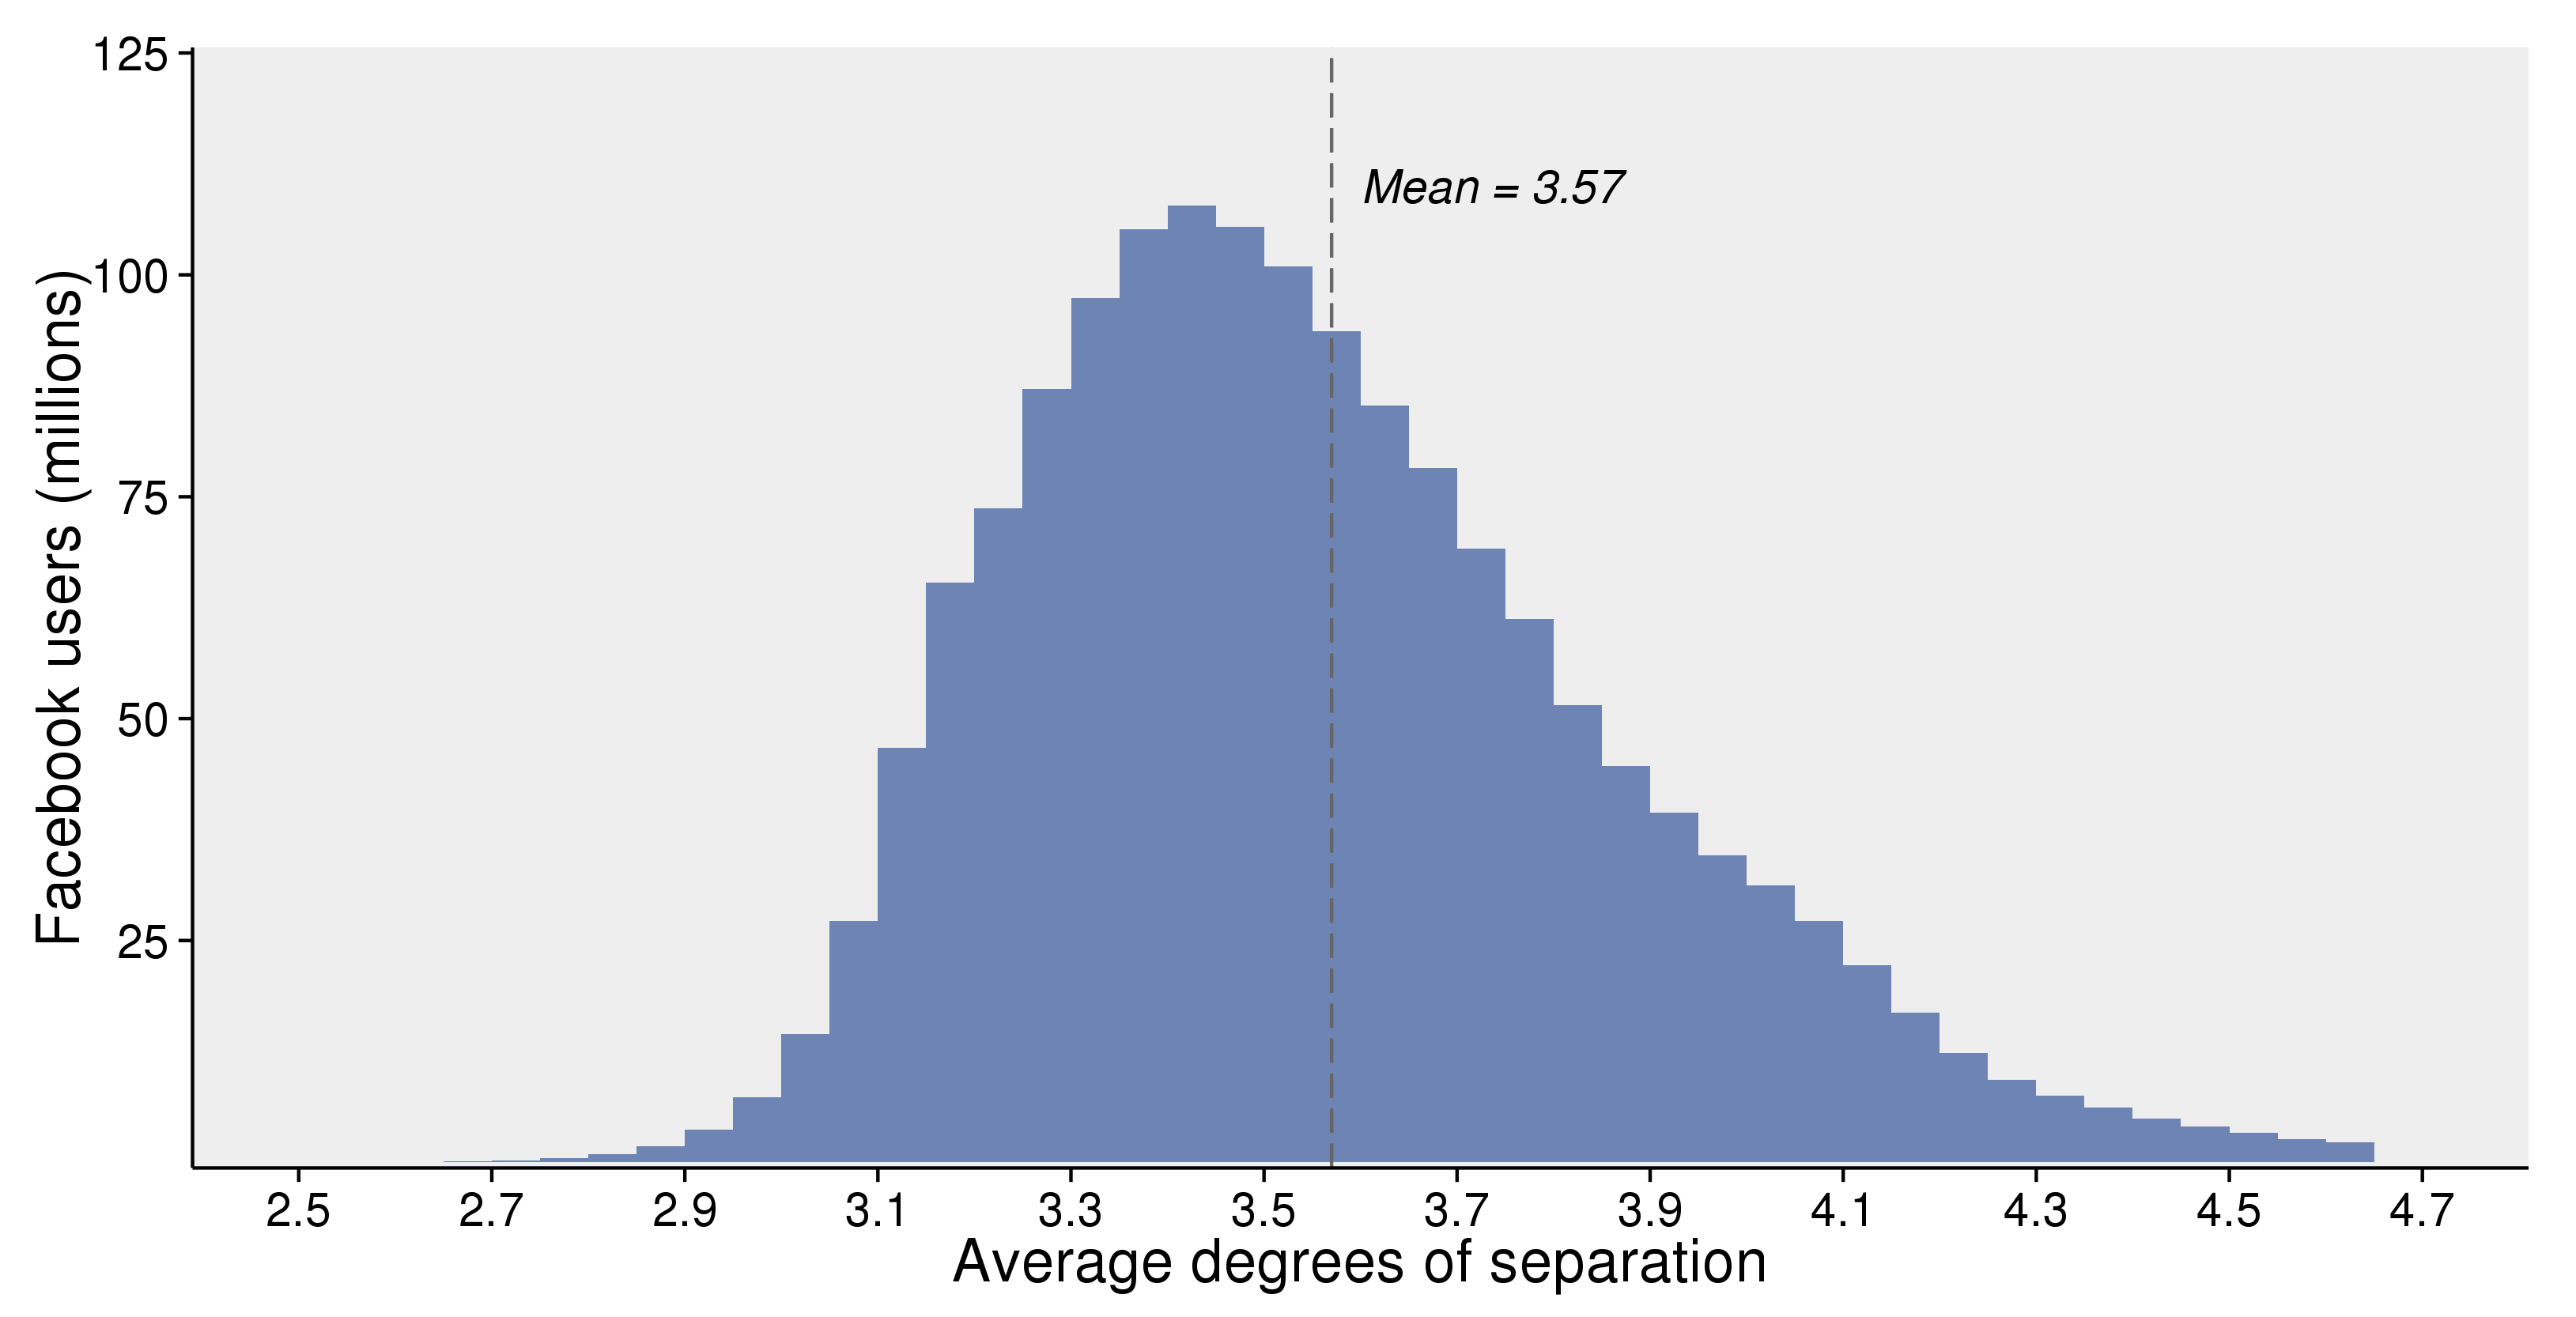
\includegraphics[width=0.9\textwidth]{images/facebook}
			\caption{In facebook la separazione media tra gli 1.6 miliardi di utenti registrati è $3.57$.\\ \textit{Fonte: facebook research, Feb 2016}}
		\end{minipage}\hfill
		%\pause
		\begin{minipage}[t]{.49\textwidth}
			\centering
			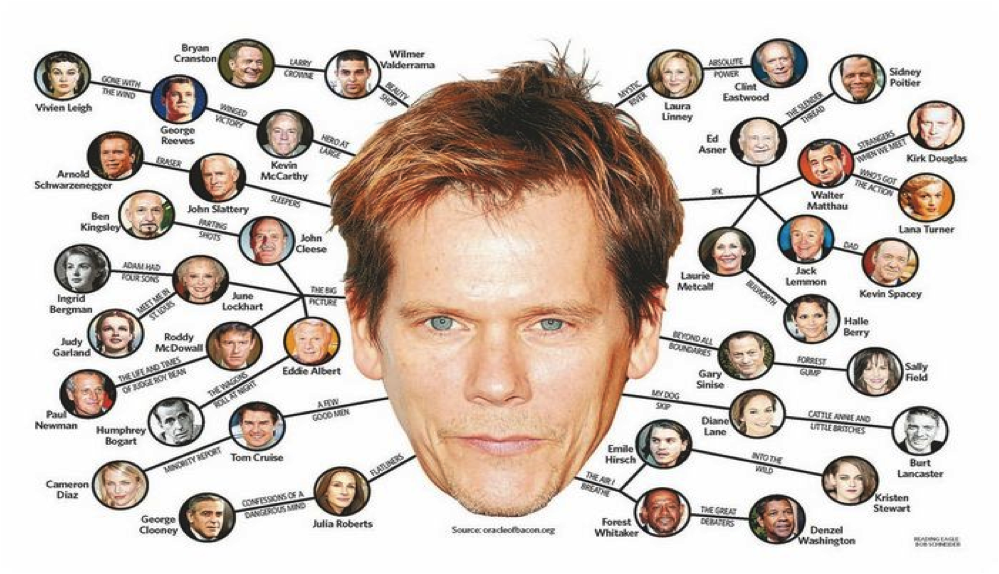
\includegraphics[width=0.9\textwidth]{images/2_kevin_bacon}
			\caption{La distanza media di collaborazioni dall'attore Kevin Bacon è $3$, il $98\%$ degli attori è a distanza minore uguale a $6$.\\ \textit{Fonte: IMDb, Ott 2017}}
		\end{minipage}
	\end{figure}
	
\end{frame}

\begin{frame}
	\frametitle{Reti etichettate e $q$-grammi}
	\centering
\end{frame}

\begin{frame}
	\frametitle{Indici di similarità}
	\centering
\end{frame}

\begin{frame}
	\frametitle{Il problema}
	\centering
\end{frame}

\begin{frame}
	\frametitle{Applicazioni pratiche}
	\centering
\end{frame}

	\section{Approcci di risoluzione}

\begin{frame}
	\sectionpage
	\centering
\end{frame}

\begin{frame}
	\frametitle{Ricerca esaustiva}

	Complessità
	\begin{itemize}
		\item Tempo: $O(|V|^q)$ $\rightarrow$ Color Coding $\rightarrow$ $O(2^{O(q)}\ |V|)$
		\item Spazio: $O(|\Sigma|^q\ q)$ $\rightarrow$ Sampling $\rightarrow$ $O(\tau q)$
	\end{itemize}
\end{frame}

\begin{frame}
	\frametitle{Color Coding}
	\centering
\end{frame}

\begin{frame}
	\frametitle{Sketching \& Sampling}
	\centering
\end{frame}

\begin{frame}
	\frametitle{F-Count}
	\centering
\end{frame}

\begin{frame}
	\frametitle{F-Samp}
	\centering
\end{frame}

\begin{frame}
	\frametitle{Baseline}
	\centering
\end{frame}

	\section{Risultati pratici}

\begin{frame}
	\Large
	\sectionpage
	\centering
\end{frame}

\begin{frame}
	\frametitle{Color Coding}
	\centering
	\Large
	Tempi di esecuzione e memoria occupata
	
	\small
	\begin{figure}[h]
		\centering
		\begin{minipage}[ht]{.49\textwidth}
			\centering
			\begin{table}
				\centering
				\begin{tabular}{|c|c|c|c|}
					\hline
					\textsc{Dataset} & $q$  &               Tempo & Memoria \\ \hline \hline
					\textsc{NetInf}  & $13$ & \phantom{11}$0.39$s & \phantom{1}$11.20$MiB     \\ \hline
					\textsc{NetInf}  & $14$ & \phantom{11}$0.81$s & \phantom{1}$22.63$MiB     \\ \hline
					\textsc{NetInf}  & $15$ & \phantom{11}$1.66$s & \phantom{1}$45.21$MiB     \\ \hline
					\textsc{NetInf}  & $16$ & \phantom{11}$3.47$s & \phantom{1}$90.93$MiB     \\ \hline \hline
					\textsc{IMDb}    & $3$  & \phantom{1}$48.22$s & \phantom{1}$17.94$MiB     \\ \hline
					\textsc{IMDb}    & $4$  &           $105.94$s & \phantom{1}$34.91$MiB     \\ \hline
					\textsc{IMDb}    & $5$  &           $241.22$s & \phantom{1}$69.01$MiB     \\ \hline
					\textsc{IMDb}    & $6$  &           $557.48$s & $137.26$MiB     \\ \hline
				\end{tabular}
			\end{table}
		\end{minipage}
		%\pause
		\begin{minipage}[ht]{.49\textwidth}
			\centering
			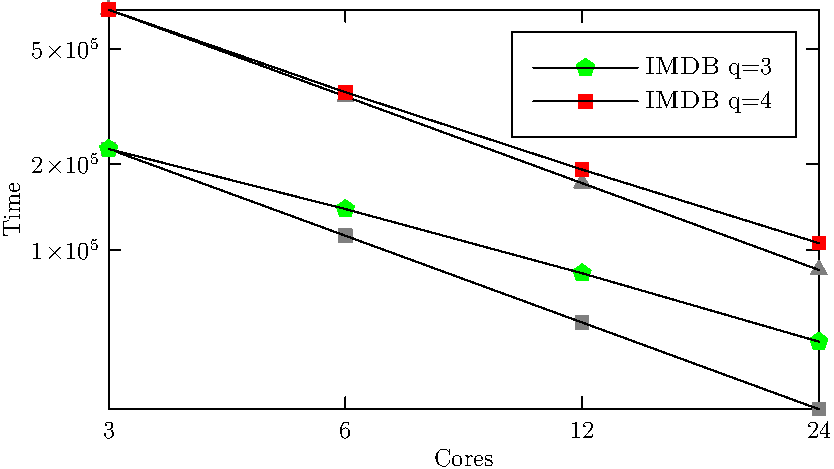
\includegraphics[width=.9\textwidth]{images/3_color_coding}
			\caption{Scalabilità al variare dei cores usati}
		\end{minipage}
	\end{figure}
	
%	Dimensione tabella 
%	\begin{table}
%		\centering
%		\begin{tabular}{|c|c|c|}
%			\hline
%			\textsc{Dataset} & $q$  & Mem. \\ \hline \hline
%			\textsc{IMDb}    & $3$  &  $17.94$MiB  \\ \hline % 34.91  / 3.49
%			\textsc{IMDb}    & $4$  &  $34.91$MiB  \\ \hline % 34.91  / 3.49
%			\textsc{IMDb}    & $5$  &  $69.01$MiB  \\ \hline % 69.01  / 8.62
%			\textsc{IMDb}    & $6$  & $137.26$MiB  \\ \hline % 137.26 / 20.58
%		\end{tabular}
%	\end{table}
	
\end{frame}

\begin{frame}
	\frametitle{Query}
	\centering
	\begin{table}[ht]
		\centering
		\begin{tabular}{|c|c|c|c|c|c|c|c|}
			\cline{6-8}
			\multicolumn{5}{c|}{} & \multicolumn{3}{c|}{Tempi (in ms)} \\ \hline
			\textsc{Dataset} & $q$ & $|A|$ & $|B|$ & $r$      & \textsc{F-Count} 	& \textsc{F-Samp} & \textsc{Base} \\ \hline \hline
			\textsc{NetInf}  & $3$ & $100$ & $100$ & $1\,000$ & $20$             	& $4$               & $2$           \\ \hline
			\textsc{NetInf}  & $3$ & $100$ & $100$ & $5\,000$ & $60$             	& $30$              & $15$          \\ \hline \hline
			\textsc{NetInf}  & $5$ & $100$ & $100$ & $1\,000$ & $2\,682$         	& $426$             & $3$           \\ \hline
			\textsc{NetInf}  & $5$ & $100$ & $100$ & $5\,000$ & $4\,767$         	& $784$             & $20$          \\ \hline \hline
			\textsc{NetInf}  & $7$ & $100$ & $100$ & $100$    & $5\,455$ 			& $4$               & $2$           \\ \hline
			\textsc{NetInf}  & $7$ & $100$ & $100$ & $200$    & $16\,634$        	& $197$             & $2$           \\ \hline \hline
			\textsc{IMDb}    & $3$ & $10$  & $10$  & $100$    & $5\,035$         	& $66$              & $1$           \\ \hline
			\textsc{IMDb}    & $4$ & $10$  & $10$  & $100$    & $/$              	& $443$             & $8$           \\ \hline
			\textsc{IMDb}    & $5$ & $10$  & $10$  & $100$    & $/$              	& $781$             & $12$          \\ \hline
			\textsc{IMDb}    & $6$ & $10$  & $10$  & $100$    & $/$              	& $1\,379$          & $14$          \\ \hline
		\end{tabular}
		\medskip
		
		Tempi per il calcolo dell'indice di Bray-Curtis
		
		$r =$ Dimensione del campione
	\end{table}
\end{frame}

\definecolor{green}{RGB}{0,200,83}
\definecolor{orange}{RGB}{255, 171, 0}
\definecolor{red}{RGB}{213,0,0}

\begin{frame}
	\frametitle{$\epsilon$-approssimazione}
	\centering
	
	Confronto a parità di livello di approssimazione $\epsilon$
	\begin{table}[ht]
	%	\centering
		\begin{tabular}{|c|c|c|c|c|c|c|c|c|c|c|}
			\cline{3-11}
			\multicolumn{2}{c|}{} & \multicolumn{3}{c|}{\fcount} & \multicolumn{3}{c|}{\fsamp} & \multicolumn{3}{c|}{\base}\\
			\hline	
			$q$ & $\epsilon$ & $r$ & T    & VAR      & $r$ & T    & VAR      & $r$ & T   & VAR      \\ \hline
			$3$ & $0.20$     & \color{green}$2$  & $1$  & $0.0725$ & \color{orange}$400$     & $1$  & $0.1194$ & \color{   red}$420$     & $1$ & $0.1150$ \\ \hline
			$3$ & $0.10$     & \color{green}$3$  & $1$  & $0.0692$ & \color{   red}$1\,000$  & $1$  & $0.0601$ & \color{orange}$900$     & $1$ & $0.1338$ \\ \hline
			$3$ & $0.05$     & \color{green}$4$  & $1$  & $0.0535$ & \color{   red}$3\,200$  & $1$  & $0.0273$ & \color{orange}$1\,500$  & $1$ & $0.1025$ \\ \hline
			\hline
			$4$ & $0.20$     & \color{green}$3$  & $2$  & $0.0677$ & \color{   red}$1\,300$  & $1$  & $0.1194$ & \color{orange}$1\,300$  & $1$ & $0.2424$ \\ \hline
			$4$ & $0.10$     & \color{green}$5$  & $4$  & $0.0532$ & \color{   red}$3\,200$  & $2$  & $0.0992$ & \color{orange}$2\,500$  & $2$ & $0.1806$ \\ \hline
			$4$ & $0.05$     & \color{green}$10$ & $8$  & $0.0518$ & \color{   red}$8\,000$  & $4$  & $0.0612$ & \color{orange}$7\,900$  & $3$ & $0.1081$ \\ \hline
			\hline
			$5$ & $0.20$     & \color{green}$5$  & $6$  & $0.0511$ & \color{orange}$5\,000$  & $4$  & $0.1678$ & \color{   red}$6\,000$  & $3$ & $0.2234$ \\ \hline
			$5$ & $0.10$     & \color{green}$10$ & $18$ & $0.0370$ & \color{orange}$20\,000$ & $12$ & $0.0745$ & \color{   red}$30\,000$ & $8$ & $0.1234$ \\ \hline
			$5$ & $0.05$     & \color{green}$20$ & $58$ & $0.0204$ & \color{orange}$80\,000$ & $30$ & $0.0376$ & \color{   red}$/$       & $/$ & $/$      \\ \hline
		\end{tabular}
		
		\medskip
			Dati riferiti all'indice di Bray-Curtis su $\textsc{NetInf}$
		\small
		\begin{flushleft}
		
		
			Dimensione sottografi $|A| = |B| = 100$
		
			$r =$ Dimensione del campione
		
			$T = $ Tempo medio elaborazione (in millisecondi)
		
			$VAR = $ Varianza indici
		
		
		\end{flushleft}

	\end{table}
\end{frame}

\begin{frame}
	\frametitle{Nella pratica}
	\centering
	\begin{table}[h]
		\centering
		\begin{tabular}{c|c|l|l}
			Attore/Attrice & Attore/Attrice  & BC index & FJ index \\ 
			\hline
			Stan Laurel    & Oliver Hardy    & 0.936167 & 0.774053 \\
			Robert De Niro & Al Pacino       & 0.730935 & 0.231474 \\
			Woody Allen    & Meryl Streep    & 0.556071 & 0.222857 \\
			Meryl Streep   & Roberto Benigni & 0.482909 & 0.160181 \\
			%\hline
		\end{tabular}
		\medskip
		
		$\textsc{IMDb}$, Similarità tra ego-network di attori famosi (F-Samp)
	\end{table}


	\begin{table}[h]
		\centering
		\begin{tabular}{c|c|l|l}
			Sito           & Sito            & BC index & FJ index \\ 
			\hline
			cnn.com      & huffpost.com  & 0.936167 & 0.774053 \\
			nytimes.com  & cnn.com       & 0.730935 & 0.231474 \\
			huffpost.com & nytimes.com   & 0.556071 & 0.222857 \\
			%\hline
		\end{tabular}
		\medskip
		
		$\textsc{NetInf}$, Similarità tra siti di informazione (F-Samp)
	\end{table}

\end{frame}

\begin{frame}
	\frametitle{Conclusioni}
	\centering
	\begin{figure}[h]
		\begin{minipage}[t]{.32\textwidth}
			\centering
			\Large
			F-Count
			\medskip

			\small		
			\textbf{Pro}:
			\begin{itemize}
				\item Accurato anche con campioni di piccole dimensioni
				\item Varianza ridotta
			\end{itemize}
		
			\textbf{Contro}:
			\begin{itemize}
				\item Lento su grafi di elevate dimensioni
				\item Preprocessing grafo (una volta sola)
			\end{itemize}
		\end{minipage}\hfill
		%\pause
		\begin{minipage}[t]{.32\textwidth}
			\centering
			\Large
			F-Samp
			\medskip
			
			\small		
			\textbf{Pro}:
			\begin{itemize}
				\item Efficiente anche in grafi di elevate dimensioni
				\item Varianza ridotta
			\end{itemize}
			
			\textbf{Contro}:
			\begin{itemize}
				\item Necessita di campioni di grandi dimensioni
				\item Preprocessing grafo (una volta sola)
			\end{itemize}
		\end{minipage}\hfill
		%\pause
		\begin{minipage}[t]{.32\textwidth}
			\centering
			\Large
			Base
			\medskip
			
			\small		
			\textbf{Pro}:
			\begin{itemize}
				\item Efficiente anche in grafi di elevate dimensioni
%				\item 
			\end{itemize}
			
			\textbf{Contro}:
			\begin{itemize}
				\item Varianza elevata
				\item Necessita di campioni di grandi dimensioni
				\item Può non convergere al valore esatto
%				\item Preprocessing grafo (una 
			\end{itemize}
		\end{minipage}\hfill
		
	\end{figure}
\end{frame}

	
	% Fine
	\section{Fine}
	\begin{frame}
		\frametitle{Fine}
		\centering
		\Large
		Grazie per l'attenzione
 	\end{frame}
 

\end{document}
